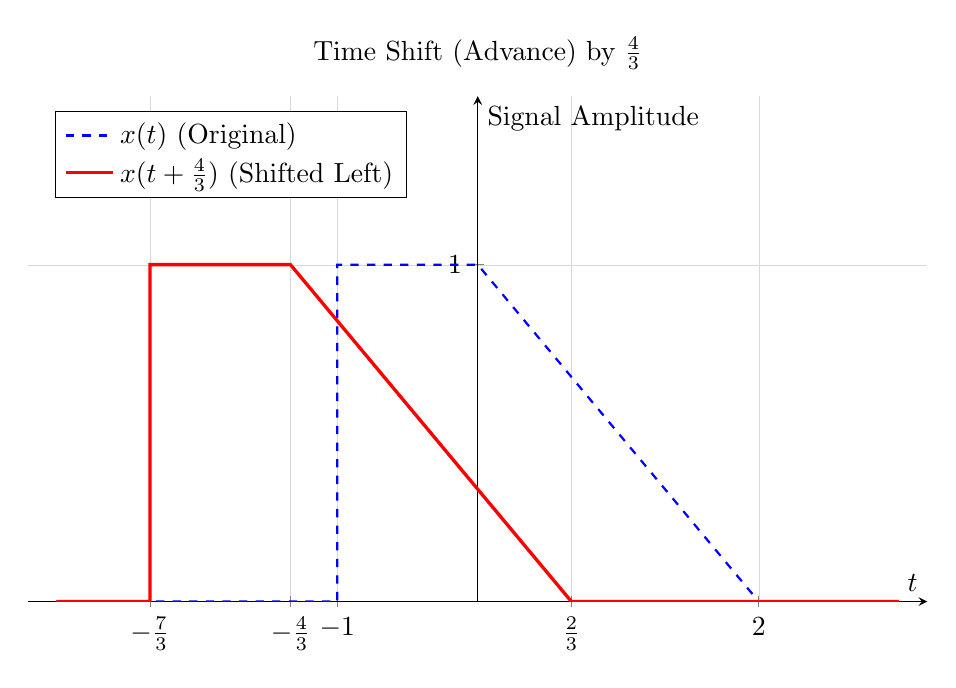
\begin{tikzpicture}
	\begin{axis}[
		% Set the overall style
		width=13cm,
		height=8cm,
		% Title and labels
		title={Time Shift (Advance) by $\frac{4}{3}$},
		xlabel={$t$},
		ylabel={Signal Amplitude},
		% Position axes at the origin
		axis lines=middle,
		% Set axis limits for good spacing
		xmin=-3.2, xmax=3.2,
		ymin=0, ymax=1.5,
		% Set ticks at key fractional and integer points
		xtick={-2.333, -1.333, -1, 0, 0.667, 2},
		% Use LaTeX to display tick labels as fractions
		xticklabels={$-\frac{7}{3}$, $-\frac{4}{3}$, $-1$, $0$, $\frac{2}{3}$, $2$},
		ytick={1},
		% Add a grid
		grid=major,
		grid style={line width=.1pt, draw=gray!30},
		% Position the legend
		legend pos=north west,
		legend cell align={left},
		]
		
		% Plot the original signal (dashed blue)
		\addplot[blue, dashed, thick] coordinates {
			(-3,0) (-1,0) (-1,1) (0,1) (2,0) (3,0)
		};
		\addlegendentry{$x(t)$ (Original)};
		
		% Plot the shifted signal (solid red)
		\addplot[red, very thick] coordinates {
			(-3,0) (-7/3,0) (-7/3,1) (-4/3,1) (2/3,0) (3,0)
		};
		\addlegendentry{$x(t + \frac{4}{3})$ (Shifted Left)};
		
	\end{axis}
\end{tikzpicture}